% !TeX spellcheck = en_US
% !TeX encoding = UTF-8

% COMPILE WITH:
% `latexmk`
% You need lualatex and biber (in all TeXLive distributions)

\documentclass[
numbers=noenddot,
fontsize=11pt,
paper=a4,
oneside,
titlepage,
bibliography=totoc,
chapterprefix=false,
DIV=calc,
headheight=14pt,
footheight=14pt,
%    draft
]{scrbook}

% LuaLaTeX-compatible font, graphics, spacing, and typography support.
\usepackage{fontspec}
\usepackage{graphicx}
\usepackage{geometry}
\geometry{a4paper,margin=2cm,includeheadfoot}
\usepackage{setspace}
\setstretch{1}
\usepackage[protrusion=false]{microtype}
\usepackage{etoolbox}
\usepackage{needspace}

% better language support
\usepackage{polyglossia}
\setdefaultlanguage{english}
\setotherlanguage{german}

\usepackage{tocbasic}
\usepackage{booktabs}
\usepackage{tikz}
\usetikzlibrary{positioning,arrows.meta}
\usepackage{tabularx}
\usepackage{multicol}
\usepackage{multirow}

\usepackage{scrlayer-scrpage}

% better bibliography (biblatex style)
% use biber to compile
\usepackage[citestyle=alphabetic, bibstyle=alphabetic, sorting=nyt, backend=biber, language=english, backref=true, maxcitenames=2]{biblatex}
% better quotes
% use \enquote{text}
\usepackage[autostyle,english=american,german=quotes]{csquotes}
\addbibresource{bibliography.bib}

% appendix
\usepackage[titletoc]{appendix}

% Allow natural line breaking in long prose, code fragments, and URLs.
\setlength{\emergencystretch}{6em}
% Keep the bibliography compact enough for the report page limit.
\AtBeginBibliography{\footnotesize\sloppy\raggedright}
\setlength{\bibitemsep}{0pt}
\setlength{\bibnamesep}{0pt}
\setlength{\bibinitsep}{0pt}
% Omit titles only for redundant online/news sources while retaining authors,
% dates, URLs, and citation information.
\AtEveryBibitem{\ifkeyword{notitle}{\clearfield{title}}{}}
\setcounter{biburlnumpenalty}{0}
\setcounter{biburlucpenalty}{0}
\setcounter{biburllcpenalty}{0}

% Compact, continuous sectioning for the requested short A4 layout.
\newcommand*{\compactchapterspace}{\par}
\AddtoDoHook{heading/preinit/chapter}{\compactchapterspace}
\RedeclareSectionCommand[beforeskip=0pt,afterskip=0.45\baselineskip]{chapter}
\RedeclareSectionCommand[beforeskip=0.75\baselineskip,afterskip=0.2\baselineskip]{section}
\RedeclareSectionCommand[beforeskip=0.5\baselineskip,afterskip=0.15\baselineskip]{subsection}
\RedeclareSectionCommand[beforeskip=0.4\baselineskip]{paragraph}
\setkomafont{chapter}{\normalfont\Large\bfseries}
\setkomafont{section}{\normalfont\large\bfseries}
\setkomafont{subsection}{\normalfont\normalsize\bfseries}
\setlength{\parindent}{0pt}
\setlength{\parskip}{0.5pt plus 0.25pt minus 0.25pt}
\setlength{\textfloatsep}{5pt plus 2pt minus 2pt}
\setlength{\floatsep}{4pt plus 2pt minus 2pt}
\setlength{\intextsep}{5pt plus 2pt minus 2pt}
\setlength{\abovecaptionskip}{2pt}
\setlength{\belowcaptionskip}{0pt}
\setcounter{topnumber}{5}
\setcounter{bottomnumber}{5}
\setcounter{totalnumber}{10}
\renewcommand{\topfraction}{0.95}
\renewcommand{\bottomfraction}{0.95}
\renewcommand{\textfraction}{0.05}
\renewcommand{\floatpagefraction}{0.8}

% where to put all images and figures
\graphicspath{{images/}{../SS/}}

% YOUR PACKAGES
\usepackage{xcolor}
\usepackage{placeins}
\usepackage{float}
\usepackage{listings}
\usepackage{subcaption}
\setmonofont{DejaVu Sans Mono}[Scale=MatchLowercase]

% Python listing style (code is included from the real source files)
\lstdefinestyle{py}{
	language=Python,
	basicstyle=\ttfamily\scriptsize,
	numbers=left,
	numberstyle=\tiny\color{gray},
	frame=tb,
	breaklines=true,
	columns=fullflexible,
	showstringspaces=false,
	keepspaces=true,
	extendedchars=true,
	keywordstyle=\color{blue!60!black},
	commentstyle=\color{green!40!black}\itshape,
	stringstyle=\color{red!50!black},
	aboveskip=4pt,
	belowskip=2pt,
	captionpos=t,
	literate=
		{→}{{\texttt{->}}}1
		{−}{{-}}1
		{≥}{{>=}}1
		{≤}{{<=}}1
		{×}{{x}}1
		{�}{{?}}1
}
\lstset{style=py}
\renewcommand{\lstlistingname}{Listing}
\captionsetup[subfigure]{font=scriptsize,skip=1pt,justification=centering}
\newcommand{\ssub}[3][0.49\linewidth]{\begin{subfigure}[t]{#1}\centering\includegraphics[width=\linewidth,height=0.3\textheight,keepaspectratio]{../SS/#2.png}\caption{#3}\label{fig:#2}\end{subfigure}}
\newcommand{\ssgrp}[3]{\begin{figure}[!htb]\centering#3\caption{#1}\label{fig:#2}\end{figure}}
\KOMAoptions{listof=nochaptergap}

% C listing style for the BPF program (Task 4) and shell style for logs (Task 5)
\lstdefinestyle{bpfc}{style=py, language=C, numbers=left, firstnumber=1, morekeywords={__u32,__u64,__u16,u32,u64}}
\lstdefinestyle{bashsh}{style=py, language=bash, numbers=none, keywordstyle=\color{black}, commentstyle=\color{green!40!black}\itshape}

% Screenshot figure: \ssfig[width]{name}{caption}; shows ../SS/<name>.png if it exists, else a framed placeholder.
\newcommand{\ssfig}[3][\linewidth]{%
	\begin{figure}[htb]
		\centering
		\IfFileExists{../SS/#2.png}{\includegraphics[width=#1,height=0.38\textheight,keepaspectratio]{../SS/#2.png}}{\fbox{\parbox{0.8\linewidth}{\centering\vspace{0.4cm}Screenshot \texttt{\detokenize{#2}}: pending\vspace{0.4cm}}}}
		\caption{#3}\label{fig:#2}
	\end{figure}}

% Title
\title{Lab 4: DDoS Defense with eBPF/XDP\\[0.4em]\Large In-Kernel Detection and Filtering}

% Author
\newcommand{\authorA}{Justlyn Kaniyanthara Johnson}
\newcommand{\authorB}{Aayush Kapoor}
\author{\authorA \& \authorB}

% Group and matriculation numbers (used on the title page)
\newcommand{\groupno}{8}
\newcommand{\matrA}{121024}
\newcommand{\matrB}{120957}

% Date
\date{\today}

% CHOOSE ACCORDINGLY
%\newcommand{\thesisType}{Bachelorarbeit}
\newcommand{\thesisType}{MasterLab}

\makeatletter
\let\thetitle\@title
\let\theauthor\@author
\let\thedate\@date
\patchcmd{\scr@startchapter}
{\if@openright\cleardoublepage\else\clearpage\fi}
{}{}
{\PackageError{compact-layout}{Continuous chapter patch failed}
	{Check the installed KOMA-Script chapter implementation.}}
\makeatother

% PDF metadata and robust links. Keep this near the end of the preamble.
\usepackage{hyperref}
\usepackage[capitalise]{cleveref}
\hypersetup{
	unicode=true,
	hidelinks,
	pdftitle={Lab 4: DDoS Defense with eBPF/XDP (in-kernel detection and filtering)},
	pdfauthor={\theauthor}
}

\pagestyle{scrheadings}
\automark[chapter]{chapter}
\chead{\leftmark}

\begin{document}
	
	%%%%%%%%%%%%%%%%%%%%%%%%%%%%%%%%%%%%%%%%%%%%%%%%%%%%%%%%%%%%%%%%%%%%%%%%%%%%%%%%%%%%%%%%%
	\frontmatter
	% CHOOSE ACCORDINGLY
	%% !TeX spellcheck = en_US
% !TeX encoding = UTF-8
\begin{titlepage}
    \centering
    \begin{onehalfspace}
    	\begin{german}
        	
\includegraphics[width=7cm]{uni-logo.png}\\
        	\vspace{1.0cm}
        	\large {\bfseries Lehrstuhl für Informatik mit Schwerpunkt\\ \textenglish{Digital Libraries and Web Information Systems}} \\

        	\vspace{2.5cm}

            \begin{doublespace}
            	\textenglish{\textsf{\Huge{\thetitle}}}
            \end{doublespace}

        	\vspace{2cm}

            \Large{Bachelorarbeit von}\\

        	\vspace{1cm}

        	{\bfseries \large{\theauthor}}

        	\vfill

        	{\large
        		\begin{tabular}[l]{cc}
        			\textsc{Prüfer}\\
        			Prof.~Dr.~Siegfried Handschuh
        		\end{tabular}
        	}

        	\vspace{1.5cm}

        	\parbox{\linewidth}{\hrule\strut}

            \vfill

	    \textgerman{\thedate}
    	\end{german}
    \end{onehalfspace}
\end{titlepage}

	% !TeX spellcheck = en_US
% !TeX encoding = UTF-8
\begin{titlepage}
    \centering
    \begin{onehalfspace}
    	\begin{german}
        	
\includegraphics[width=7cm]{uni-logo.png}\\
        	\vspace{1.0cm}
        	\large {\bfseries Security Insider Lab I}\\ 

        	\vspace{2.5cm}

            \begin{doublespace}
            	\textenglish{\textsf{\Huge{\thetitle}}}
            \end{doublespace}

        	\vspace{2cm}

			{\large Group \groupno}

        	\vspace{1cm}

        	\vfill

        	{\large
        		\begin{tabular}[l]{ll}
        			\authorA & \matrA \\
        			\authorB & \matrB \\
        			
        		\end{tabular}
        	}

        	\vspace{1.5cm}

        	\parbox{\linewidth}{\hrule\strut}

            \vfill

	    \textgerman{\thedate}
    	\end{german}
    \end{onehalfspace}
\end{titlepage}

	
	\tableofcontents
	
	% -- ABSTRACT
	% !TeX encoding = UTF-8
\chapter*{Abstract}

In the fourth lab of the Security Insider Lab, we build a complete real-time DDoS defense cycle with eBPF/XDP in which the classifier and the filter run inside the Linux kernel. One XDP program captures packets at the network driver hook, computes ten forward-direction flow features per flow in a kernel map, classifies the flow with a Decision Tree (depth 6) and an XGBoost model (20 trees, depth 4) stored in BPF maps, and drops all packets of a source that is classified as malicious. User space only trains and exports the models, loads and configures the program, and displays results. On the 33,463 test flows of the CIC-IDS2017 Friday DDoS file, the integer models reach an F1 score of 0.9991 (Decision Tree, 4 false alarms, 32 missed attacks) and 0.9989 (XGBoost, 11 false alarms, 31 missed attacks). Their verdicts agree with the floating-point models on all test flows, and the kernel code reproduces the Python integer evaluator exactly on 1,024 test vectors. In a Docker topology with an inline IDS gateway in front of Nginx and Apache, normal client traffic produced no malicious verdict and no drop, and a stub model that always answers malicious showed the filter dropping 55 packets of the normal client. Without attack tools, 60 dataset flows replayed through the attached kernel program were handled correctly: all 30 DDoS flows were classified malicious and blocked, and none of the 30 benign flows. We also configured xdp-filter and xdpdump (Task 1), built a web interface (Task 3) and containerized Nginx, Apache and a pinging container (Task 4). The models are essentially a payload-size rule, which we discuss together with the other limits of the in-kernel design.

	
	% -- Acknowledgements (optional, left out)
	% % !TeX spellcheck = en_US
% !TeX encoding = UTF-8
\chapter*{Acknowledgments}

% I would first like to thank my thesis advisor ...
	% \newpage
	
	% -- List of figures
{\footnotesize\setlength{\parskip}{0pt}
\listoffigures
\listoftables
\lstlistoflistings}
	
	%%%%%%%%%%%%%%%%%%%%%%%%%%%%%%%%%%%%%%%%%%%%%%%%%%%%%%%%%%%%%%%%%%%%%%%%%%%%%%%%%%%%%%%%%
	\mainmatter
	
	% -- Chapters
	% following IMRaD structure
	% adjust for your liking
	% !TeX encoding = UTF-8
\chapter{Introduction}\label{chap:introduction}

In the fourth lab of the Security Insider Lab, we move the DDoS detection of Lab~3 from user space into the Linux kernel. A flow classifier that runs in a Python process sees a packet only after the kernel has received, queued and copied it. The eXpress Data Path (XDP) \cite{hoiland2018xdp} runs a small, verified eBPF program at the earliest point of the receive path, before the network stack allocates its packet structures. A program at this hook can read a packet, update state in kernel maps and drop the packet at once. The lab has four tasks:

\begin{enumerate}\setlength\itemsep{0pt}
	\item \textbf{Task 1:} configure the xdp-tools collection \cite{xdptools_github} and run example commands of \texttt{xdp-filter} and \texttt{xdpdump}.
	\item \textbf{Task 2:} build a real-time cycle: capture packets, compute flow features, classify each flow, and filter it. We chose the \emph{best case} of the task sheet: the classifier \emph{and} the filter both run in the kernel, inside one XDP program. User space only loads the models, configures the program and displays results.
	\item \textbf{Task 3:} build a web interface with an interface selector, a timespan, a start button and a table with the algorithm output.
	\item \textbf{Task 4:} run Nginx, Apache and a pinging container in Docker and check that they can communicate.
\end{enumerate}

\paragraph{Scope and rules.} The task sheet forbids attacking tools in the real-time test. We therefore show the filter without any attack tool: with normal client traffic, with a stub model that always answers \enquote{malicious}, and by replaying flows of the dataset through the attached kernel program (Section~\ref{sec:replay}). The classifier is a Decision Tree (DT), an XGBoost model (XGB), or both (\texttt{--model DT|XGB|ALL}).

\paragraph{Data.} We use the Friday-afternoon DDoS file of CIC-IDS2017 \cite{sharafaldin2018cicids} with the cleaning and the 70/15/15 stratified split of Lab~3: 225,745 raw flows become 223,082 after removing 34 rows with infinite or missing values and 2,629 duplicates, and the split gives 156,157 training, 33,462 validation and 33,463 test flows (test: 19,202 DDoS, 14,261 benign; \texttt{outputs/metrics/preprocess\_summary.json}). Labels are BENIGN\,=\,0 and DDoS\,=\,1.

\paragraph{Structure.} Chapter~\ref{chap:task2} is the core of the report; Appendix~\ref{app:repro} lists the commands to reproduce everything. Every number comes from files under \texttt{outputs/} or from the metadata of \texttt{models/kernel\_model.json}; the file is named in the caption or the text.

	% !TeX encoding = UTF-8
\chapter{Task 1: xdp-tools}\label{chap:task1}

\section{Installation}
xdp-tools \cite{xdptools_github} is a collection of utilities around libxdp. We built the source tree (version \texttt{v1.6.3-32-g92a9828}) and installed it with \texttt{make \&\& sudo make install \&\& sudo ldconfig}. The binaries (\texttt{xdp-loader}, \texttt{xdp-filter}, \texttt{xdpdump}, \texttt{xdp-bench}) go to \texttt{/usr/local/sbin}, libxdp to \texttt{/usr/local/lib} and the BPF objects of xdp-filter to \texttt{/usr/local/lib/bpf}. We deliberately did not install a second copy from the distribution packages, because two copies on the \texttt{PATH} would conflict.

\section{Sandbox}
xdp-filter attaches a program to an interface, and a wrong rule on the main uplink can lock a remote user out. All Task~1 commands therefore run in a sandbox that \texttt{xdp\_tools/task1\_demo.sh} creates and removes: a network namespace \texttt{lab4t1} with a veth pair. The host end \texttt{t1-host} (10.10.0.1/24) carries the XDP program in generic (skb) mode; the other end \texttt{t1-ns} (10.10.0.2/24) lives in the namespace. A \texttt{trap} unloads xdp-filter, stops the test web server and deletes the namespace and the veth pair when the script ends, also after an error. The script prints ten numbered sections, one per screenshot. The commands are the examples of the xdp-filter and xdpdump READMEs with the interface name replaced.

\section{xdpdump: listing and loading}
\texttt{xdpdump -D} lists the interfaces and the XDP programs attached to them. In Figure~\ref{fig:SS_T1_1} nothing is loaded. \texttt{xdp-filter load --mode skb t1-host} attaches the filter; \texttt{xdp-filter} uses libxdp's dispatcher, so the next \texttt{xdpdump -D} shows \texttt{xdp\_dispatcher} with the filter program behind it (Figure~\ref{fig:SS_T1_2}). With no rule defined the filter passes all packets, and a ping from the namespace shows 0\,\% loss (Figure~\ref{fig:SS_T1_3}).

\ssgrp{Task 1, sections 1--3: loading the filter.}{grpT1a}{\ssub{SS_T1_1}{Section 1: \texttt{xdpdump -D}, no XDP program loaded.}\hfill\ssub{SS_T1_2}{Section 2: after \texttt{xdp-filter load}, the dispatcher and filter program are listed.}}
\ssgrp{Task 1, sections 3--4: ping without and with the source-IP rule.}{grpT1b}{\ssub{SS_T1_3}{Section 3: the ping passes (0\,\% loss) while the filter has no rule.}\hfill\ssub{SS_T1_4}{Section 4: with the source-IP rule the ping loses all packets; \texttt{status} shows the rule and counters.}}

\section{xdp-filter: IP and port rules}
\texttt{xdp-filter ip 10.10.0.2 -m src} adds the namespace address as a blocked \emph{source} address. The next ping loses all packets, and \texttt{xdp-filter status} lists the address with non-zero hit counters (Figure~\ref{fig:SS_T1_4}). The rule is removed with \texttt{-r}, after which the ping works again (Figure~\ref{fig:SS_T1_5}).

For a port rule, a Python web server runs inside the namespace on 10.10.0.2:8000. A request from the host returns HTTP 200. After \texttt{xdp-filter port 8000 -m src} the request times out, because the replies carry source port 8000 and enter \texttt{t1-host}; \texttt{status} shows the port, and after the removal the request returns 200 again (Figure~\ref{fig:SS_T1_6}).


\section{xdpdump: capturing at the XDP hook}
\texttt{xdpdump} attaches itself to the program already running on the interface. With \texttt{--rx-capture=entry,exit} it records every packet twice: at program entry and at program exit together with the action the program returned. While the IP rule is active, the exit records show \texttt{XDP\_DROP} (Figure~\ref{fig:SS_T1_5}). Option \texttt{-x} prints a hex dump of each packet (Figure~\ref{fig:SS_T1_7_1}, \ref{fig:SS_T1_7_2}). Writing a pcap stream to standard output and piping it into \texttt{tcpdump -r - -n} decodes the same packets as ICMP echo requests and replies (Figure~\ref{fig:SS_T1_8}).

\ssgrp{Task 1, sections 5--6: capture at the hook and the port rule.}{grpT1c}{\ssub{SS_T1_5}{Section 5: \texttt{xdpdump --rx-capture=entry,exit} shows the exit action \texttt{XDP\_DROP}; after the rule is removed the ping works.}\hfill\ssub{SS_T1_6}{Section 6: port filter: HTTP 200, timeout while the rule exists, \texttt{status}, HTTP 200 after removal.}}
\ssgrp{Task 1, section 7: \texttt{xdpdump -x}.}{grpT1d}{\ssub{SS_T1_7_1}{Hex dump of the packets seen at the XDP hook (start of the output).}\hfill\ssub{SS_T1_7_2}{Further packets.}}
\ssgrp{Task 1, sections 8--10: pcap pipe, poll counters and unload.}{grpT1e}{\ssub[0.52\linewidth]{SS_T1_8}{Section 8: \texttt{xdpdump -w - | tcpdump -r - -n} decodes the captured packets.}\hfill\ssub[0.45\linewidth]{SS_T1_9}{Section 9: \texttt{xdp-filter poll -i 1000}, counters per action for five seconds.}\\[3pt]\ssub[0.52\linewidth]{SS_T1_10}{Section 10: after \texttt{xdp-filter unload} no program is loaded.}}

\section{xdp-filter poll and unload}
\texttt{xdp-filter poll -i 1000} prints the packet and byte rates per XDP action once per second. Figure~\ref{fig:SS_T1_9} shows 16 packets counted as \texttt{XDP\_DROP} and a slowly growing \texttt{XDP\_PASS} count in every period of the five-second run. Finally \texttt{xdp-filter unload t1-host} removes the program, and \texttt{xdpdump -D} shows nothing loaded again (Figure~\ref{fig:SS_T1_10}).


xdp-filter is a ready-made, \emph{static} filter: it drops by address or port rules that an operator adds. It has no notion of a flow and no classifier. Task~2 builds what is missing for DDoS defense: a filter whose rules the kernel program writes itself, from a per-flow classification.
\FloatBarrier
	% !TeX encoding = UTF-8
\chapter{Task 2: Real-Time Cycle in the Kernel}\label{chap:task2}

\section{Architecture}\label{sec:arch}
The cycle has four steps: capture, flowmeter, classification and filtration. In our best-case design all four run in one XDP program, \texttt{xdp\_ids} (\texttt{xdp/lab4\_xdp.bpf.c}), attached to the interface \texttt{ext0} of an IDS container that acts as an inline gateway between a client and two web servers (Figure~\ref{fig:arch}; the Docker setup is in Chapter~\ref{chap:task4}).

\begin{figure}[htb]
\centering
\begin{tikzpicture}[font=\footnotesize, node distance=5mm and 7mm, >=Stealth,
  box/.style={draw, rounded corners=2pt, minimum height=7mm, align=center},
  stage/.style={draw, fill=blue!8, minimum height=6mm, minimum width=3.6cm, align=center},
  ]
  \node[stage] (s1) {1 capture: XDP hook, \texttt{ext0}};
  \node[box, left=8mm of s1] (client) {client\\172.28.1.20};
  \node[stage, below=2mm of s1] (s2) {2 blocklist: source blocked? $\to$ \texttt{XDP\_DROP}};
  \node[stage, below=2mm of s2] (s3) {3 flowmeter: per-flow counters (map)};
  \node[stage, below=2mm of s3] (s4) {4 classify: DT / XGB trees (maps)};
  \node[stage, below=2mm of s4, fill=red!10] (s5) {5 filter: malicious $\to$ block source, drop};
  \node[box, right=14mm of s3] (fwd) {\texttt{XDP\_PASS}\\forward\\\texttt{int0}};
  \node[box, right=8mm of fwd, yshift=7mm] (ng) {nginx\\172.28.2.10};
  \node[box, below=2mm of ng] (ap) {apache\\172.28.2.11};
  \node[box, below=10mm of s5, xshift=-10mm] (ua) {user space (same container): \texttt{agent.py} / \texttt{webui.py} $\to$ \texttt{bpftool}};
  \node[box, left=8mm of ua] (br) {browser (host)\\\texttt{mgmt0}:8080};
  \draw[->] (client) -- (s1);
  \draw[->] (s1) -- (s2); \draw[->] (s2) -- (s3); \draw[->] (s3) -- (s4); \draw[->] (s4) -- (s5);
  \draw[->] (s3.east) -- (fwd.west);
  \draw[->] (fwd.east) -- ++(2mm,0) |- (ng.west);
  \draw[->] (fwd.east) -- ++(2mm,0) |- (ap.west);
  \draw[<->, dashed] (s5.south) -- ++(0,-3mm) -| (ua.north);
  \draw[<->, dashed] (br) -- (ua);
\end{tikzpicture}
\caption{Data path of the best case. Stages 1 to 5 are one XDP program; the models and the blocklist are kernel maps that user space fills and reads through \texttt{bpftool}.}\label{fig:arch}
\end{figure}

\begin{enumerate}\setlength\itemsep{0pt}
	\item \textbf{Capture.} The program sees every frame of \texttt{ext0} before the IP stack. IPv4 TCP and UDP packets are parsed with bounds checks; ARP, IPv6, ICMP, fragments, VLAN frames and malformed packets pass untouched and are counted.
	\item \textbf{Blocklist.} If the source address is in the \texttt{blocklist} map and the entry has not expired, the packet is dropped. Expired entries are deleted on the next packet of that source.
	\item \textbf{Flowmeter.} A least-recently-used hash map \texttt{flows} keeps one record per 5-tuple with packet and byte counters, the packet length extremes and the inter-arrival times.
	\item \textbf{Classification.} At certain packets of a flow (below) the program computes the ten features of Section~\ref{sec:features} and walks the integer trees stored in the maps \texttt{nodes} and \texttt{roots}.
	\item \textbf{Filtration.} A malicious verdict writes the source into the blocklist for \texttt{--block-seconds} (default 60\,s) and drops the packet. All internal errors fail open: the packet passes.
\end{enumerate}

\section{Kernel features}\label{sec:features}
XDP runs on ingress only. In our topology the program therefore sees the client-to-server packets of a flow, the \emph{forward} direction, and never the replies. CICFlowMeter, which produced the dataset, also computes backward and bidirectional features (flow duration, bytes per second, backward packet lengths). Computing them differently in the kernel would silently change their meaning, so we use only ten forward-direction features that the kernel computes exactly with integer arithmetic (Table~\ref{tab:features}).

\begin{table}[htb]
\centering\small
\begin{tabular}{@{}rllr@{}}
\toprule
Idx & CIC column & Kernel computation (forward packets) & Scale\\
\midrule
0 & Total Fwd Packets & packet count & 1\\
1 & Total Length of Fwd Packets & sum of L4 payload bytes & 1\\
2 & Fwd Packet Length Max & largest payload & 1\\
3 & Fwd Packet Length Min & smallest payload & 1\\
4 & Fwd Packet Length Mean & bytes\,$\cdot$\,1000 / packets & 1000\\
5 & Fwd IAT Total & last $-$ first timestamp (ns) & 1000\\
6 & Fwd IAT Mean & (last $-$ first) / (packets $-$ 1) & 1000\\
7 & Fwd IAT Max & largest gap & 1000\\
8 & Fwd IAT Min & smallest gap & 1000\\
9 & act\_data\_pkt\_fwd & packets with payload $>0$ & 1\\
\bottomrule
\end{tabular}
\caption{The ten kernel features (\texttt{xdp/lab4\_common.h}, \texttt{common.KERNEL\_FEATURES}). The dataset stores inter-arrival times in microseconds and the kernel measures nanoseconds, hence scale 1000. All divisions are unsigned integer divisions.}\label{tab:features}
\end{table}

The payload length is the IPv4 total length minus the IP and the TCP or UDP header, never the frame length, so Ethernet padding is not counted. We left out two features that score highly in Lab~2 and Lab~3 but are shortcuts: the \emph{destination port} (nearly all DDoS flows of the file go to port 80, which is exactly the port of our demo web servers, so a port-based model would flag normal demo traffic) and \emph{Init\_Win\_bytes\_forward} (a fingerprint of the 2017 attack hosts). We also left out the standard-deviation features, which need an integer square root and CICFlowMeter's conventions, and the header-length features with known CICFlowMeter quirks. The cost in accuracy is small (Section~\ref{sec:training}).

\section{Integer decision trees}\label{sec:int}
eBPF has no floating-point arithmetic. Trees are invariant to feature scaling, so we train on the \emph{raw} feature values (no scaler) and convert the thresholds. Features and thresholds are integers in kernel units: $x_{\mathrm{int}}=\lfloor x\cdot s\rfloor$ with the scale $s$ of Table~\ref{tab:features}. A sklearn tree goes left if $x\le t$, so $T=\lfloor t\cdot s\rfloor$. XGBoost goes left if $x<t$ for a float32 threshold $t$, so $T=\lceil t\cdot s\rceil-1$. In both cases the kernel rule is the same: \emph{left iff} $x_{\mathrm{int}}\le T$.

A Decision Tree leaf is class 1 if $P(\mathrm{DDoS})>0.5$. An XGBoost leaf value is stored as a fixed-point integer $\mathrm{round}(\mathrm{leaf}\cdot 2^{16})$; the base score becomes a margin $\mathrm{round}(\mathrm{logit}(b)\cdot 2^{16})$. The verdict is malicious if the margin sum is positive (an exact zero is normal, matching the rule $\mathrm{score}>0.5$). The exported model has 387 nodes in total (\texttt{models/kernel\_model.json}, key \texttt{meta}). Each node is 24 bytes (\texttt{struct tree\_node}); the maps hold up to 8,192 nodes and 64 trees. The decision tree root is \texttt{roots[0]}, the XGBoost trees are \texttt{roots[1..20]}.

\section{The XDP program}\label{sec:xdp}
Listing~\ref{lst:walk} is the core of the classifier: a bounded loop that follows node indices in the \texttt{nodes} map. The constant bound lets the verifier prove termination, and each map lookup is checked for \texttt{NULL}. XGBoost sums its 20 trees with the helper \texttt{bpf\_loop}, and \texttt{classify} (Listing~\ref{lst:classify}) combines the verdicts: with \texttt{ALL} the flow is malicious only if both models say so, because the action is a drop and a false drop costs more than a missed detection in this demo.

\lstinputlisting[style=bpfc,linerange={108-129},caption={\texttt{walk\_tree}: integer tree walk (\texttt{xdp/lab4\_xdp.bpf.c}).},label={lst:walk}]{../xdp/lab4_xdp.bpf.c}
\lstinputlisting[style=bpfc,linerange={168-188},caption={\texttt{classify}: DT, XGB or both models must agree (\texttt{xdp/lab4\_xdp.bpf.c}).},label={lst:classify}]{../xdp/lab4_xdp.bpf.c}

\paragraph{When a flow is classified.} The dataset rows describe \emph{completed} flows, while a SYN-only partial flow looks like a one-packet flow, which is something else. The kernel therefore classifies a flow at a packet with the FIN or RST flag, and re-checks long or connectionless flows when the packet count is a power of two and at least 8 (8, 16, 32, \ldots). Flows with fewer than 8 packets and no FIN or RST are never classified. Listing~\ref{lst:block} shows the blocklist check and the filter step.

\lstinputlisting[style=bpfc,linerange={310-317,353-361},caption={Essentials of \texttt{xdp\_ids}: the blocklist check at the start, and the filter step (a malicious verdict blocks the source and drops the packet).},label={lst:block}]{../xdp/lab4_xdp.bpf.c}

\section{User space with bpftool}
User space contains no custom loader. The agent (\texttt{script/agent.py}) calls \texttt{bpftool} with an argument list (never through a shell): \texttt{prog loadall} with pinned maps, one \texttt{batch} file with all node, root and config updates, \texttt{net attach xdpgeneric}, JSON map dumps that carry BTF-formatted values, and \texttt{prog run} for tests. The program is attached only \emph{after} the model and the configuration are in the maps, and always detached on exit. Once per second the agent dumps the \texttt{flows} and \texttt{stats} maps and prints one JSON line per classified flow. A per-interface file lock allows one capture per interface. The interface name is validated against \texttt{/sys/class/net}, the management interface is refused, and the timespan and model are range-checked. The command line is \texttt{agent.py --iface ext0 --model \{DT,XGB,ALL\} --timespan S --block-seconds B --replay N} (\texttt{--replay} 0 to 100, default 0).

\section{Training and depth selection}\label{sec:training}
We port the cleaning and the 70/15/15 split of Lab~3, so the test split holds the same rows, and then keep the ten kernel features. The models are \texttt{DecisionTreeClassifier} and \texttt{XGBClassifier} (20 trees, learning rate 0.1, no early stopping, so exactly 20 trees go to the kernel). The depth is chosen on the \emph{validation} split: the smallest depth whose validation F1 is within 0.0005 of the best (Table~\ref{tab:depth}). The test split is used once.

\begin{table}[htb]
\centering\small
\begin{tabular}{@{}llrrr@{}}
\toprule
Model & Depth & 4 & 5 & 6 \\
\midrule
XGBoost (20 trees) & val F1 & 0.99896 & 0.99906 & 0.99904 \\
\bottomrule
\end{tabular}\\[3pt]
\begin{tabular}{@{}llrrr@{}}
\toprule
Model & Depth & 6 & 8 & 10 \\
\midrule
Decision Tree & val F1 & 0.99904 & 0.99914 & 0.99906 \\
\bottomrule
\end{tabular}
\caption{Validation F1 per depth (\texttt{outputs/metrics/depth\_selection.json}). Selected: DT depth 6, XGB depth 4.}\label{tab:depth}
\end{table}

Table~\ref{tab:metrics} gives the test results. We report all four counts and F1, not accuracy alone. The \emph{integer} rows are the models as the kernel evaluates them.

\begin{table}[htb]
\centering\small
\begin{tabular}{@{}lrrrrrrrrr@{}}
\toprule
Model & Acc & Prec & Rec & F1 & ROC-AUC & TP & TN & FP & FN \\
\midrule
Decision Tree (d6) & 0.9989 & 0.9998 & 0.9983 & 0.9991 & 0.9999 & 19170 & 14257 & 4 & 32 \\
XGBoost (20 trees, d4) & 0.9987 & 0.9994 & 0.9984 & 0.9989 & 0.9998 & 19171 & 14250 & 11 & 31 \\
Decision Tree (integer) & 0.9989 & 0.9998 & 0.9983 & 0.9991 & 0.9990 & 19170 & 14257 & 4 & 32 \\
XGBoost (integer) & 0.9987 & 0.9994 & 0.9984 & 0.9989 & 0.9998 & 19171 & 14250 & 11 & 31 \\
\bottomrule
\end{tabular}
\caption{Test metrics on 33,463 flows (\texttt{outputs/metrics/comparison\_test.md}); DDoS is the positive class. The integer Decision Tree outputs hard classes, hence its lower ROC-AUC.}\label{tab:metrics}
\end{table}

The kernel models keep the F1 within about 0.001 of the 59-feature models of Lab~3 (XGBoost F1 1.0000 there), although they see 10 forward-only features and 387 nodes. The integer models have the same confusion matrices as the floating-point models. Table~\ref{tab:imp} shows why so few features suffice: two payload-size features carry about 99\,\% of the importance.

\begin{table}[htb]
\centering\small
\begin{tabular}{@{}lrr@{}}
\toprule
Feature & DT importance & XGB gain importance \\
\midrule
Total Length of Fwd Packets & 0.4205 & 0.2784 \\
Fwd Packet Length Max & 0.5765 & 0.7185 \\
all other eight features, each & $\le 0.0011$ & $\le 0.0012$ \\
\bottomrule
\end{tabular}
\caption{Feature importance (\texttt{outputs/metrics/feature\_importance.md}; the full table lists all ten).}\label{tab:imp}
\end{table}

\section{Verification chain}\label{sec:verify}
We check three links. First, \texttt{train.py} compares the floating-point predictions with a Python integer evaluator on all 33,463 test rows: the verdicts agree on 100\,\% of the rows for both models (0 mismatches), and the largest margin error of XGBoost is $4.5\cdot 10^{-5}$ (\texttt{outputs/metrics/parity.json}, \texttt{ac\_pass} true). Second, a second program \texttt{classify\_test} in the same object evaluates 1,024 test vectors in the kernel (\texttt{BPF\_PROG\_TEST\_RUN}); the DT verdicts and XGB margins equal the Python integer evaluator exactly. Third, kernel tests run the real program on crafted packets: flowmeter counts, classification trigger, blocklist, block expiry, mode \texttt{ALL} needs both models, mode off, and the pass-through of ARP, IPv6, ICMP, fragments, short packets, bad header lengths and VLAN frames. \texttt{outputs/kernel/kernel\_tests.log} reports 18 passing kernel tests (Figure~\ref{fig:SS_DOCKER_IDS}). Together, the kernel decides what the trained model decides.

\ssfig[0.6\linewidth]{SS_DOCKER_IDS}{Kernel tests in the IDS image (\texttt{docker run --privileged}, 18 passed).}

\paragraph{Size and cost.} The verifier accepts \texttt{xdp\_ids}: 5,664 bytes of translated and 3,263 bytes of JIT-compiled code (\texttt{outputs/kernel/prog\_sizes.json}). Table~\ref{tab:timing} lists the average run time per packet measured with \texttt{BPF\_PROG\_TEST\_RUN}. Untracked packets cost almost nothing, packets in the middle of a flow only update counters, and the walk of the 20 XGBoost trees is the most expensive step. Classification happens once per flow (at FIN) or at power-of-two packet counts, not for every packet.

\begin{table}[htb]
\centering\small
\begin{tabular}{@{}lrrr@{}}
\toprule
Packet (ns per run) & DT & XGB & ALL \\
\midrule
not tracked (ARP etc.) & \multicolumn{3}{c}{18} \\
mid-flow (counters only) & 61 & 82 & 60 \\
classifying (FIN) & 120 & 366 & 542 \\
\bottomrule
\end{tabular}
\caption{Average time per \texttt{BPF\_PROG\_TEST\_RUN} (\texttt{outputs/kernel/timing.json}).}\label{tab:timing}
\end{table}

\section{Live cycle}\label{sec:live}
In the Docker topology, a client requests the two web servers once per second through the IDS gateway, normal traffic only. Table~\ref{tab:live} lists the runs. In 60-second runs with DT, XGB and ALL, the program classified 118 flows each, none of them malicious, and dropped no packet. Each classified flow had 5 to 7 packets and was classified at its FIN (Figure~\ref{fig:SS_T2_3} shows the \texttt{ALL} output; the DT and XGB modes work the same way and were also run, Table~\ref{tab:live} has their numbers). The counter \texttt{ST\_PASS} also counts untracked packets, so it can exceed \texttt{ST\_PKTS}.

\begin{table}[htb]
\centering\small
\begin{tabular}{@{}lrrrrrrr@{}}
\toprule
Run & Time (s) & Packets & Classified & Malicious & Drops & Blocks & Untracked \\
\midrule
DT, normal traffic & 60 & 703 & 118 & 0 & 0 & 0 & 3 \\
XGB, normal traffic & 60 & 701 & 118 & 0 & 0 & 0 & 2 \\
ALL, normal traffic & 60 & 710 & 118 & 0 & 0 & 0 & 1 \\
DT, stub model, block 20\,s & 30 & 66 & 2 & 2 & 55 & 2 & 2 \\
\bottomrule
\end{tabular}
\caption{Live runs on \texttt{ext0} (\texttt{outputs/realtime/20261125-225252\_ext0\_DT\_summary.json}, \ldots\texttt{225354\_ext0\_XGB}, \ldots\texttt{225456\_ext0\_ALL}, \ldots\texttt{225602\_ext0\_DT}).}\label{tab:live}
\end{table}

\ssfig{SS_T2_3}{Agent CLI with \texttt{--model ALL}: one JSON line per classified flow, both verdicts listed (client 172.28.1.20 to the two servers, all Normal).}

\paragraph{Filter without attack tools.} With a good model and normal traffic the filter never fires. To show it anyway, we ran the agent with a stub model (\texttt{tests/fixtures/always\_malicious.json}: one decision-tree leaf with value 1) and a 20-second block time. The first classified flow of the client blocked its source, 55 packets were dropped in 30 seconds, and the source was blocked a second time after the first block expired (the last row of Table~\ref{tab:live}). Figure~\ref{fig:SS_T2_5} shows the client: requests fail with a timeout while the source is blocked and succeed between blocks.

\ssfig[0.45\linewidth]{SS_T2_5}{Client log during the filter demo: \texttt{FAIL} lines (timeouts) while the client is blocked, \texttt{OK} lines in between.}

\section{Replay of dataset flows}\label{sec:replay}
Real attack traffic is not allowed, so we push dataset flows through the \emph{same attached kernel program}. \texttt{train.py} writes \texttt{models/replay\_flows.json}, a pool of 1,000 flows (500 benign, 500 DDoS) of the \emph{test} split whose forward packets can be rebuilt exactly: at most 32 packets, and a list of payload sizes that reproduces the packet count, the total, maximum, minimum, mean and active-packet count. With \texttt{--replay N} (UI default 20) the session draws $N/2$ benign and $N/2$ DDoS flows at random and injects them at random times spread over the first 80\,\% of the capture (each poll tick injects the flows that are due), so they interleave with live flows. Each flow is rebuilt as TCP packets from a random source in 10.99.0.0/16 to 172.28.2.10:80, with FIN and ACK on the last packet, and injected with \texttt{bpftool prog run} into the pinned \texttt{xdp\_ids} program. The real flowmeter, models and blocklist therefore produce the verdicts, and the rows appear in the same table as live flows. Nothing is sent on the wire, and blocks only affect 10.99.x.y.

\paragraph{Limit.} Packets run through \texttt{BPF\_PROG\_TEST\_RUN} are microseconds apart, so the inter-arrival features of a replayed flow do not reproduce the dataset. These features carry less than 0.5\,\% of the importance (Table~\ref{tab:imp}), but the replay is not a test of timing behaviour.

\paragraph{Results.} A kernel test replays 50 DDoS and 50 benign flows: all 50 DDoS flows are classified malicious, none of the benign flows (\texttt{outputs/kernel/replay\_summary.json}). In three live captures with mode \texttt{ALL} (\texttt{outputs/realtime/20261126-*\_ext0\_ALL\_replay.json}) the replayed flows were handled as follows.

\begin{table}[htb]
\centering\small
\begin{tabular}{@{}lrrrr@{}}
\toprule
Capture & DDoS replayed & DDoS dropped & Benign replayed & Benign dropped \\
\midrule
20261126-180119 & 30 & 30 & 30 & 0 \\
20261126-180431 & 30 & 30 & 30 & 0 \\
20261126-180721 & 13 & 13 & 17 & 0 \\
\bottomrule
\end{tabular}
\caption{Replay in live captures with \texttt{--model ALL} (\texttt{outputs/realtime/*\_replay.json}); a flow counts as dropped if one of its packets returned \texttt{XDP\_DROP}.}\label{tab:replay}
\end{table}

These flows come from the test split, so the result repeats the high within-day scores of Table~\ref{tab:metrics} in the live program, with the exact flow reconstruction as the only difference.

\section{Proof that classifier and filter run in the kernel}\label{sec:proof}
During a capture with replayed flows, the following views show that the decision is made in the kernel. Pins live under \texttt{/sys/fs/bpf/lab4/ext0/} and disappear when the capture ends.

\ssgrp{Kernel proof, part 1: attach, program and detach.}{grpK1}{\ssub{SS_K_1}{\texttt{bpftool net show dev ext0}: the XDP program is attached to \texttt{ext0} in generic mode.}\hfill\ssub{SS_K_7}{After the capture, \texttt{bpftool net show dev ext0} lists no XDP program: detached cleanly.}\\[3pt]\ssub[0.8\linewidth]{SS_K_2}{\texttt{bpftool prog show name xdp\_ids}: the verified and JIT-compiled program (5,664 B translated, 3,263 B JIT).}}
\ssgrp{Kernel proof, part 2: maps and counters.}{grpK2}{\ssub{SS_K_3}{Pinned maps, \texttt{config} and \texttt{nodes}: mode \texttt{ALL}, 20 XGBoost trees, and the root node of the decision tree stored in the kernel.}\hfill\ssub{SS_K_5}{\texttt{blocklist} map dump: each key is a blocked source IPv4 read as a little-endian 32-bit number (e.g.\ 4272710410 = 10.99.172.254, also Malicious in Figure~\ref{fig:SS_K_6}), the value its expiry time in ns.}\\[3pt]\ssub[0.95\linewidth]{SS_K_4}{Counters kept by the program: classified flows, malicious flows, blocks added and dropped packets are all above zero.}}
\ssgrp{Kernel proof, part 3: verdicts.}{grpK3}{\ssub[0.95\linewidth]{SS_K_6}{Agent output (or the UI table) with Malicious rows from the replayed DDoS flows.}}
\FloatBarrier
	% !TeX encoding = UTF-8
\chapter{Task 3: Front-End Interface}\label{chap:task3}

The sample on the task sheet shows a dark page with a dropdown of local interfaces, a timespan field, a \emph{Start Packet Capture} button and a table called \emph{Algorithm Output} with source and destination address and port, a timestamp and the result (Normal or Malicious). We built the same page (\texttt{web/index.html}, one file with HTML, CSS and JavaScript, no external libraries) and a small server (\texttt{script/webui.py}, Python standard library only) that uses the same \texttt{Session} class as the command-line agent.

\section{Controls and API}
\begin{itemize}\setlength\itemsep{0pt}
	\item \textbf{Available Local Interfaces:} filled from \texttt{GET /api/interfaces}. The management interface \texttt{mgmt0} is hidden, so the page cannot attach a program to the interface that carries its own traffic. The default is \texttt{ext0}.
	\item \textbf{Enter Timespan:} seconds, 1 to 3600.
	\item \textbf{Model:} DT, XGB or ALL (we added this dropdown to the sample).
	\item \textbf{Replay dataset flows:} number of test-split flows replayed through the kernel program at random times over the first 80\,\% of the capture, interleaved with live flows (default 20, 0 to 100; Section~\ref{sec:replay}).
	\item \textbf{Start Packet Capture / Stop:} \texttt{POST /api/start} answers 202, 400 for invalid input or 409 if a capture is already running on the interface; \texttt{POST /api/stop} ends it.
	\item \textbf{Status line and table:} the page polls \texttt{GET /api/flows}. The status line shows the remaining time and the counters (packets, dropped, classified, malicious, blocks). Malicious rows are red. The Models column shows the verdict of each model.
\end{itemize}
The server validates every field (interface, timespan, model, a request body of at most 4\,KB). It listens only on the management address 172.28.0.2:8080, so the browser on the host can reach it, but the client behind the XDP hook cannot, and its own polling never crosses \texttt{ext0}.

\section{Screenshots}
Each capture replays 20 dataset flows (half benign, half DDoS), so the table holds at least 20 rows with a random mix of Normal and Malicious, together with the live client flows (172.28.1.20). Figure~\ref{fig:SS_T3_3} shows the ALL capture: the status line reads 335 packets, 8 dropped, 55 classified, 7 malicious and 7 blocks. The DT and XGB captures look the same and were also run. The blocked sources are replayed 10.99.x.y addresses, and the client 172.28.1.20 stays Normal.

\begin{figure}[H]
	\centering
	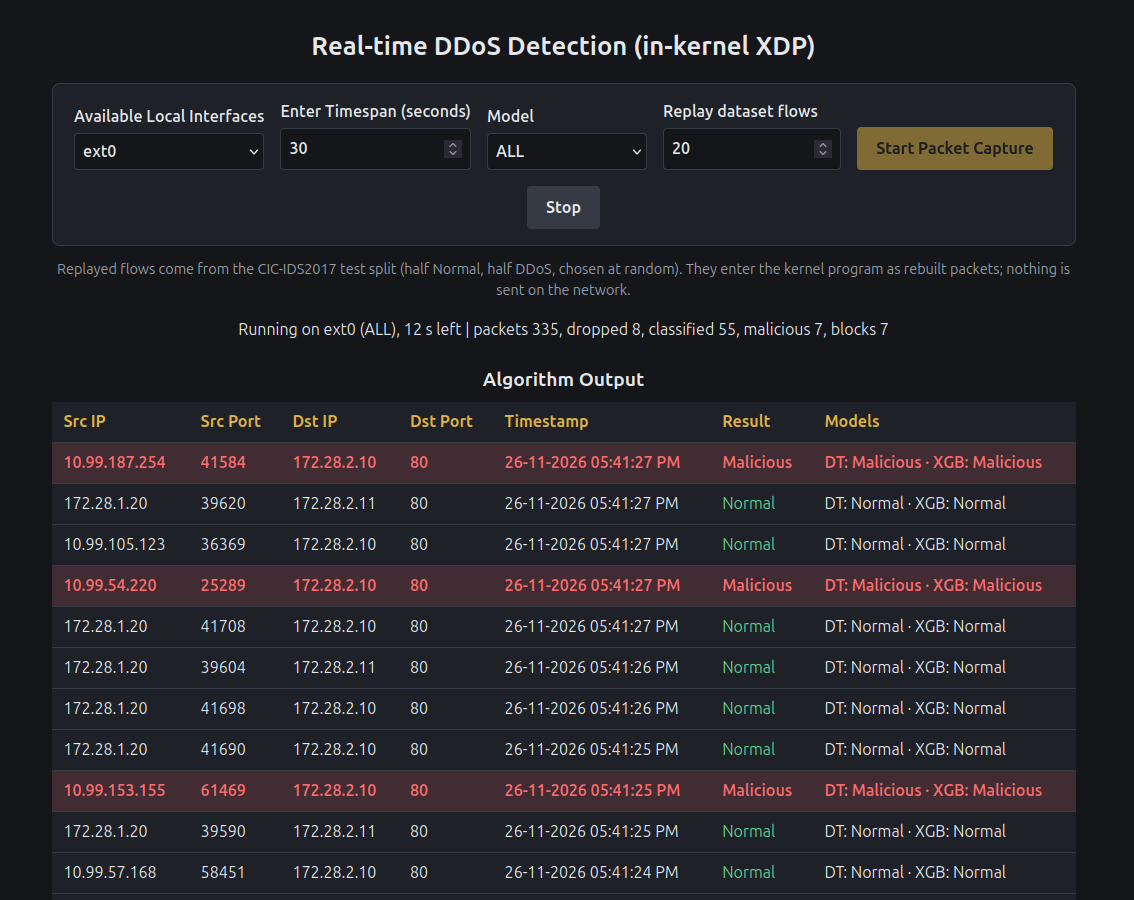
\includegraphics[width=0.85\linewidth,height=0.38\textheight,keepaspectratio]{../SS/SS_T3_3.png}
	\caption{Web interface with both models (\texttt{ALL}): Malicious rows need both verdicts.}\label{fig:SS_T3_3}
\end{figure}
\FloatBarrier
	% !TeX encoding = UTF-8
\chapter{Task 4: Containerization}\label{chap:task4}

Task~4 asks for Docker containers for Nginx and Apache and a container that pings both, and to check whether they can communicate. \texttt{docker-compose.yml} (project \texttt{lab4}) starts these three services and also the IDS gateway and the normal-traffic client that Tasks~2 and~3 need. Table~\ref{tab:topo} lists the networks and services, Figure~\ref{fig:arch} shows the data path.

\begin{table}[htb]
\centering\small
\begin{tabular}{@{}lllll@{}}
\toprule
Service & Image & Network (IP, interface) & Role \\
\midrule
\texttt{nginx} & \texttt{nginx:stable-alpine} & back: 172.28.2.10 & web server (Task 4)\\
\texttt{apache} & \texttt{httpd:2.4-alpine} & back: 172.28.2.11 & web server (Task 4)\\
\texttt{pinger} & \texttt{alpine:3} & back: 172.28.2.30 & pings both servers (Task 4)\\
\texttt{client} & \texttt{alpine:3} & front: 172.28.1.20 & normal HTTP traffic via the IDS\\
\texttt{ids} & \texttt{lab4-ids:latest} & mgmt: 172.28.0.2 (\texttt{mgmt0}) & UI and agent\\
 & & front: 172.28.1.2 (\texttt{ext0}) & XDP hook\\
 & & back: 172.28.2.2 (\texttt{int0}) & forwarding with NAT\\
\bottomrule
\end{tabular}
\caption{Compose topology (\texttt{docker-compose.yml}). Networks: \texttt{mgmt} 172.28.0.0/24, \texttt{front} 172.28.1.0/24, \texttt{back} 172.28.2.0/24.}\label{tab:topo}
\end{table}

The IDS container is privileged (loading BPF needs CAP\_BPF, CAP\_NET\_ADMIN and CAP\_SYS\_ADMIN; membership of the \texttt{docker} group is root-equivalent, which is acceptable for a lab machine). It owns its network namespace, so XDP can never touch the host uplink, and removing the container removes the program, the pins and all blocks. The \texttt{interface\_name} option gives the three interfaces fixed names, and the client reaches the servers through the IDS via a route to 172.28.2.0/24 through 172.28.1.2. The image builds the BPF object in a build stage (clang, libbpf) and ships only \texttt{bpftool}, \texttt{iproute2}, \texttt{iptables} and the Python scripts in the runtime stage, so it contains no numpy or scikit-learn.

\section{Communication check}
\texttt{docker/task4\_check.sh} runs from the pinger: three pings each to \texttt{nginx} and \texttt{apache} by name and to 172.28.2.10 and 172.28.2.11 by address, and an HTTP request to each server. All checks pass (\texttt{outputs/task4/task4\_check.log} ends with \texttt{RESULT: all checks PASSED}; ping round trips are below 1\,ms with 0\,\% loss). Figure~\ref{fig:SS_T4_1} shows the running services and Figure~\ref{fig:SS_T4_2} the check.

\ssgrp{Task 4: running services and communication check.}{grpT4}{\ssub[0.52\linewidth]{SS_T4_1}{\texttt{docker compose ps}: all five services are up.}\hfill\ssub[0.42\linewidth]{SS_T4_2}{\texttt{docker/task4\_check.sh}: ping by name and IP, HTTP to Nginx and Apache.}}

	\FloatBarrier
	% !TeX encoding = UTF-8
\chapter{Discussion}\label{chap:discussion}

\paragraph{What the results show.} A decision tree and a 20-tree XGBoost model fit into one XDP program of 5,664 translated bytes, and the kernel reproduces the Python integer models exactly. A classification costs between about 120\,ns (DT) and 366\,ns (XGB); mode ALL runs both models and costs about their sum (542\,ns) in the measurement of Table~\ref{tab:timing}. The F1 scores of 0.9991 and 0.9989 are within about 0.001 of the models of Lab~3 that use 59 features, although the kernel models use ten.

\paragraph{The model is a payload-size rule.} Two features, the largest forward payload and the total forward payload, carry about 99\,\% of the importance (Table~\ref{tab:imp}). The Friday DDoS flows are an HTTP flood with a characteristic request size, and the trees learned that size. The high F1 therefore says that this attack is easy to separate by request size within the test split. It says little about other attacks or other networks, and the live demo traffic (small \texttt{wget} requests) happens to fall on the normal side. We did not tune the thresholds for the demo. Had normal flows come out malicious, we would have reported it instead of changing features.

\paragraph{Ingress only.} XDP runs on receive, so the program sees only the forward direction. Backward and bidirectional features (flow duration, bytes per second, backward packet lengths) are absent, because computing them differently from CICFlowMeter would change their meaning (Section~\ref{sec:features}).

\paragraph{Partial flows.} CICFlowMeter rows describe completed flows. The kernel classifies at FIN or RST and at power-of-two packet counts from 8 on, so a flow with fewer than 8 packets and no FIN or RST (for example a short UDP exchange) is never classified, and a source can send many such flows unblocked. A timer-based idle expiry would close this gap and is out of scope. A reused 5-tuple continues the old flow entry, which is rare with ephemeral ports. Flow counters are not atomic across CPUs, which is accepted at demo rates.

\paragraph{No attack tools.} The task sheet forbids attacking tools. The filter is therefore shown with a stub model on normal traffic and with the dataset replay. The replay (Section~\ref{sec:replay}) does not reproduce inter-arrival times and uses test-split flows, so it does not measure robustness against a new attack. Classifier performance on live malicious traffic was not checked, as the sheet allows.

\paragraph{Other limits.} Only IPv4 TCP and UDP are inspected; everything else passes. The program runs in generic (skb) mode, because native mode on veth needs extra setup. The privileged container is root-equivalent. The consensus rule of \texttt{ALL} drops fewer flows than either model alone, so a flow that only one model flags is passed. Remedies such as multi-day training data or more features were not part of this lab.

	% !TeX encoding = UTF-8
\chapter{Conclusion}\label{chap:conclusion}

We built the best case of the real-time cycle: one XDP program that captures packets, keeps per-flow features in a kernel map, classifies flows with a Decision Tree and an XGBoost model stored in BPF maps, and drops all traffic of a source that is classified as malicious. User space only trains, exports and configures. The integer models match the floating-point models on all 33,463 test flows and the kernel matches the Python evaluator exactly on 1,024 vectors; the test F1 is 0.9991 (DT) and 0.9989 (XGB). In the Docker gateway topology, normal traffic caused no drop, a stub model showed the filter blocking the client, and 60 replayed dataset flows were handled correctly, all 30 DDoS flows blocked and none of the 30 benign flows. Task~1 documented xdp-filter and xdpdump in a sandbox, Task~3 provides the interface, and Task~4 shows that Nginx, Apache and the pinger communicate. The main limit is the narrow basis of the classifier: it is essentially a request-size rule from one attack file.

	
	\begin{appendices}
		% !TeX encoding = UTF-8
\chapter{Reproduction}\label{app:repro}

All commands run from \texttt{Lab4/}. The complete, step-by-step list is in \texttt{README.md} and \texttt{USER\_COMMANDS\_RUN.md}; \texttt{bash run.sh} runs training, build and kernel tests in one go.

\begin{lstlisting}[style=bashsh]
uv venv --python 3.12 .venv && uv pip install --python .venv/bin/python -r requirements.txt
.venv/bin/python script/train.py          # clean, split, depth selection, train, export, parity
.venv/bin/pytest -m "not kernel and not docker" -q
make -C xdp && docker compose build ids
docker run --rm --privileged -v "$PWD/models:/lab4/models:ro" lab4-ids:latest \
    python3 -m pytest tests/test_kernel.py -m kernel -q
docker compose up -d && bash docker/task4_check.sh
docker compose exec ids python3 script/agent.py --iface ext0 --model ALL --timespan 30
sudo bash xdp_tools/task1_demo.sh 2>&1 | tee xdp_tools/logs/task1_demo.log
\end{lstlisting}

The web interface opens at \texttt{http://172.28.0.2:8080} on the host. The kernel-proof screenshots (Section~\ref{sec:proof}) use \texttt{agent.py --replay 60} with the \texttt{bpftool} commands of Section~7 of \texttt{USER\_COMMANDS\_RUN.md}.

	\end{appendices}
	
		% -- Appendix (optional, left out for now: the template's Code/Math/Dataset chapters are empty)
	% \begin{appendices}
		%     \input{appendix.tex}
		% \end{appendices}
	% \newpage
	
	
	%%%%%%%%%%%%%%%%%%%%%%%%%%%%%%%%%%%%%%%%%%%%%%%%%%%%%%%%%%%%%%%%%%%%%%%%%%%%%%%%%%%%%%%%%
	\backmatter
	
	% -- Bibliography
	\printbibliography
	
	% -- Eidesstattliche Erklärung (= Affadavit)
	\clearpage
	% !TeX spellcheck = de_DE
% !TeX encoding = UTF-8
\begin{german}
\chapter{Eidesstattliche Erklärung}

	Hiermit versichere ich, dass ich diese \thesisType{} selbstständig und ohne Benutzung anderer als der angegebenen Quellen und Hilfsmittel angefertigt habe und alle Ausführungen, die wörtlich oder sinngemäß übernommen wurden, als solche gekennzeichnet sind, sowie, dass ich die \thesisType{} in gleicher oder ähnlicher Form noch keiner anderen Prüfungsbehörde vorgelegt habe.

	\vspace{3cm}

	Passau, \thedate

	\vspace{2cm}

	\parbox{7cm}{\hrule \strut Justlyn Kaniyanthara Johnson}
	\hfill
	\parbox{7cm}{\hrule \strut Aayush Kapoor}
\end{german}

	
	
\end{document}
